%% BioMed_Central_Tex_Template_v1.06
%%                                      %
%  bmc_article.tex            ver: 1.06 %
%                                       %

%%IMPORTANT: do not delete the first line of this template
%%It must be present to enable the BMC Submission system to
%%recognise this template!!

%%%%%%%%%%%%%%%%%%%%%%%%%%%%%%%%%%%%%%%%%
%%                                     %%
%%  LaTeX template for BioMed Central  %%
%%     journal article submissions     %%
%%                                     %%
%%          <8 June 2012>              %%
%%                                     %%
%%                                     %%
%%%%%%%%%%%%%%%%%%%%%%%%%%%%%%%%%%%%%%%%%


%%%%%%%%%%%%%%%%%%%%%%%%%%%%%%%%%%%%%%%%%%%%%%%%%%%%%%%%%%%%%%%%%%%%%
%%                                                                 %%
%% For instructions on how to fill out this Tex template           %%
%% document please refer to Readme.html and the instructions for   %%
%% authors page on the biomed central website                      %%
%% http://www.biomedcentral.com/info/authors/                      %%
%%                                                                 %%
%% Please do not use \input{...} to include other tex files.       %%
%% Submit your LaTeX manuscript as one .tex document.              %%
%%                                                                 %%
%% All additional figures and files should be attached             %%
%% separately and not embedded in the \TeX\ document itself.       %%
%%                                                                 %%
%% BioMed Central currently use the MikTex distribution of         %%
%% TeX for Windows) of TeX and LaTeX.  This is available from      %%
%% http://www.miktex.org                                           %%
%%                                                                 %%
%%%%%%%%%%%%%%%%%%%%%%%%%%%%%%%%%%%%%%%%%%%%%%%%%%%%%%%%%%%%%%%%%%%%%

%%% additional documentclass options:
%  [doublespacing]
%  [linenumbers]   - put the line numbers on margins

%%% loading packages, author definitions

%\documentclass[twocolumn]{bmcart}% uncomment this for twocolumn layout and comment line below
\documentclass{bmcart}

%%% Load packages
%\usepackage{amsthm,amsmath}
%\RequirePackage{natbib}
%\RequirePackage{hyperref}
\usepackage[utf8]{inputenc} %unicode support
\usepackage{url}
\usepackage{graphics}
\usepackage{graphicx}
%\usepackage[applemac]{inputenc} %applemac support if unicode package fails
%\usepackage[latin1]{inputenc} %UNIX support if unicode package fails


%%%%%%%%%%%%%%%%%%%%%%%%%%%%%%%%%%%%%%%%%%%%%%%%%
%%                                             %%
%%  If you wish to display your graphics for   %%
%%  your own use using includegraphic or       %%
%%  includegraphics, then comment out the      %%
%%  following two lines of code.               %%
%%  NB: These line *must* be included when     %%
%%  submitting to BMC.                         %%
%%  All figure files must be submitted as      %%
%%  separate graphics through the BMC          %%
%%  submission process, not included in the    %%
%%  submitted article.                         %%
%%                                             %%
%%%%%%%%%%%%%%%%%%%%%%%%%%%%%%%%%%%%%%%%%%%%%%%%%


%\def\includegraphic{}
%\def\includegraphics{}



%%% Put your definitions there:
%\startlocaldefs
%\endlocaldefs


%%% Begin ...
\begin{document}

\begin{frontmatter}

\begin{fmbox}
\dochead{Research}

\title{An Investigation of the Performance of UK ISP Web Filters}

\author[
   addressref={lancs},                   % id's of addresses, e.g. {aff1,aff2}
   corref={lancs},                       % id of corresponding address, if any
   %noteref={n1},                        % id's of article notes, if any
   email={m.rowe@lancaster.ac.uk}   % email address
]{\inits{MR}\fnm{Matthew} \snm{Rowe}}
\author[
   addressref={org},                   % id's of addresses, e.g. {aff1,aff2}
   corref={org},                       % id of corresponding address, if any
   %noteref={n1},                        % id's of article notes, if any
   email={richard@openrightsgroup.org}   % email address
]{\inits{RK}\fnm{Richard} \snm{King}}

\address[id=lancs]{%                           % unique id
  \orgname{Data Science Group, School of Computing and Communications}, % university, etc
  \street{Lancaster University},                     %
  \postcode{LA1 4WA}                                % post or zip code
  \city{Lancaster},                              % city
  \cny{UK}                                    % country
}
\address[id=org]{%                           % unique id
  \orgname{Open Rights Group}, % university, etc
  \street{Free Word Centre, 60 Farringdon Road},                     %
  \postcode{EC1R 3GA}                                % post or zip code
  \city{London},                              % city
  \cny{UK}                                    % country
}

\end{fmbox}% comment this for two column layout

\begin{abstractbox}

\begin{abstract} % abstract
To do
\end{abstract}


\begin{keyword}
\kwd{sample}
\kwd{article}
\kwd{author}
\end{keyword}

% MSC classifications codes, if any
%\begin{keyword}[class=AMS]
%\kwd[Primary ]{}
%\kwd{}
%\kwd[; secondary ]{}
%\end{keyword}

\end{abstractbox}
%
%\end{fmbox}% uncomment this for twcolumn layout

\end{frontmatter}

%%%%%%%%%%%%%%%%%%%%%%%%%%%%%%%%%%%%%%%%%%%%%%
%%                                          %%
%% The Main Body begins here                %%
%%                                          %%
%% Please refer to the instructions for     %%
%% authors on:                              %%
%% http://www.biomedcentral.com/info/authors%%
%% and include the section headings         %%
%% accordingly for your article type.       %%
%%                                          %%
%% See the Results and Discussion section   %%
%% for details on how to create sub-sections%%
%%                                          %%
%% use \cite{...} to cite references        %%
%%  \cite{koon} and                         %%
%%  \cite{oreg,khar,zvai,xjon,schn,pond}    %%
%%  \nocite{smith,marg,hunn,advi,koha,mouse}%%
%%                                          %%
%%%%%%%%%%%%%%%%%%%%%%%%%%%%%%%%%%%%%%%%%%%%%%

%%%%%%%%%%%%%%%%%%%%%%%%% start of article main body
% <put your article body there>

%%%%%%%%%%%%%%%%
%% Background %%
%%
\section*{Introduction}

%Context/Problem
%-Introduction of UK ISP Web Filters
%-Questions over:
%--the need for this (cite ofcom survey states)
%--their accuracy, given that the ISPs use third-party systems or categorisations
%--how they can be held to account
%--who is responsible for their oversight (this is left vague)

In 2013, the United Kingdom government instructed all UK-based Internet Service Providers (ISPs) to provide new customers with an `\textit{unavoidable}' choice: \textit{to turn on web filtering, or not}. 
This was presented to such customers as a web-based form to which the customers provided their answer; and should the customer select \textit{yes} then for certain ISPs additional questions would be asked about the level of filtering required.
Such web filtering was mandated in order to protect children from adult content (e.g. pornography, alcohol, and drugs), and to ensure that they can browse and use the Web in a safe manner.
However after one year of the provision of such filters, an Ofcom report\footnote{\url{http://stakeholders.ofcom.org.uk/internet/internet-safety-2}} found that for new ISP customers, who were offered the choice of filtering uptake ranged across ISPs from only 5\% to 36\%.

During the period since the filters inception, various news outlets have reported on examples of `\textit{overblocking}' by ISPs - where sites are blocked that should not have been - such as sexual health advice blogs, charity web sites, addiction-support sites, and politics-related web sites and opinion blogs.
This has led to questions being raised as to the accuracy of the filters, what they are blocking that they should not be (\textit{overblocking}), and what sites they are not filtering out that they should be (\textit{underblocking}); in sum, calling into question the \textit{efficacy} of the filters and the degree of censorship that they are enabling.
Despite such questions being raised, little is known of how effective the filters are, as the ISPs do not report on their accuracy.
Motivated by this current lack of understanding, in this paper we investigate the following three research questions:

\begin{enumerate}
	\item \textbf{RQ1}: How can we understand how UK ISP Web Filters function, and how accurate they are?
	\item \textbf{RQ2}: How reliable are the filters at blocking content, in terms of both overblocking and underblocking across different categories of sites? And are there certain categories of web sites that are error prone?
	\item \textbf{RQ3}: How long does it take an ISP to fix an error?
\end{enumerate}

In order to investigate the above questions, we present a study of both UK ISPs and Mobile Service Providers' (MSPs) filters using data collected by the Open Rights Group\footnote{A non-profit UK-based organisation who campaign for and work to promote digital rights} as part of their Blocked.org.uk\footnote{\url{https://www.blocked.org.uk/}} project.
The aim of the project was to \textit{probe} a range of Internet (ISPs) and Mobile Service Providers (MSPs) with a collection of URLs and collect examples of blocked web sites.
We follow a \textit{data science} approach by first performing exploratory analysis at the \textit{macro} level of what domains are commonly blocked and what categories of sites are blocked by the filters, before then investigating the accuracy of the filters and to identify any categories of sites that are routinely \textit{overblocked} and \textit{underblocked} - thereby performing a relational study of filters and site categories.

This work is the first to investigate the performance of UK ISP web filters and to provide evidence of both overblocking and underblocking.
For that reason, the work has implications for the domain of digital rights and censorship, and also data science in the methodology that we follow in investigating web filters' performance through data.









\section*{Related Work}
-Explain existing studies of web censorship
--Explain how the UK approach is different as it is via UK ISPs and therefore pushed out to the private sector

\section*{Studied Internet Service Providers}
-Explain which internet service providers are included
--Different blocking settings used and analysed (e.g. BT moderate, BT strict, etc.)
-Explain what |SPs use which companies services

\subsection*{Analysed Internet Service Providers}

\subsubsection*{Broadband Providers}
-BT
-Plusnet
-Sky
-TalkTalk
-VirginMedia

\subsubsection*{Mobile Providers}
-EE
-O2
-T-Mobile
-VirginMobile
-Vodafone

\subsubsection*{Blocking Approaches}
-BT: 
--provides a system known as `BT-parent controls'\footnote{\url{http://www.productsandservices.bt.com/products/manage-broadband-extras/}} which uses DNS-based blocking of URLs
--uses site categorisation information from Nominum
--Provides three levels of filtering once controls are turned on: (i) light, which blocks pornography, obscene and tasteless, hate and self-harm, drugs, alcohol and tobacco, and dating; (ii) moderate, which blocks all of the light filter setting's content and nudity, weapons and violence, gambling, and social networking, and finally; (iii) strict, which blocks all of the above plus fashion and beauty, file-sharing, games, and media streaming.

-Plusnet
--provides a system known as `Plusnet Protect'

-Sky
--provides a system known as `Sky Broadband Shield'  which also uses DNS-based blocking of URLs
--uses site categorisation information provided Symantec and their Rulespace Web Content categorisation system\footnote{\url{http://www.symantec.com/page.jsp?id=rulespace}} 
--Also offers three levels of categorisation: (i) 18 which blocks malware sites; (ii) 13 which blocks cyber-bullying, pornography, suicide and self-harm, drugs, dating, and malware sites, and; (iii) PG which blocks all of the above plus social networking and online gaming.

-Talk Talk
--Talk Talk Homesafe
--Uses DPI to examine URLs being visited by users. Sites blocked using DNS-spoofing
--Includes setting of 'Kids-Safe' filter that allows certain categories of sites to be blocked: "Dating", "Drugs, Alcohol and Tobacco", "File Sharing Sites", "Gambling", "Games", "Pornography", "Social Networking", "Suicide and Self-Harm", "Weapons and Violence".


-VirginMedia: provides a system known as `Web Safe'\footnote{\url{http://my.virginmedia.com/my-apps/websafe.html}} which is a DNS-based system that matches requested URLs with known blocked URLs in a DNS-lookup table.
--uses site categorisation information from Nominum
--Data was not immediately available of what VirginMedia blocks, therefore used the OFCOM Internet Safety Measures report.

Good overview of which categories the filters cover is included in the OFCOM Internet Safety Measures report from 2014.\footnote{\url{http://stakeholders.ofcom.org.uk/binaries/internet/internet_safety_measures_2.pdf}}


\clearpage
\section*{Monitoring Web Filters}
-Explain the framework that was used for this
-Explain the submission interface and the use of the blocked portal to check what has been blocked and unblocked
-Gathering evidence of overblocking and underblocking
-Show the distribution of requests per day per ISP filter

\begin{figure}[h!]
\caption{\csentence{Number of URL requests made over time since the beginning of the project.}}
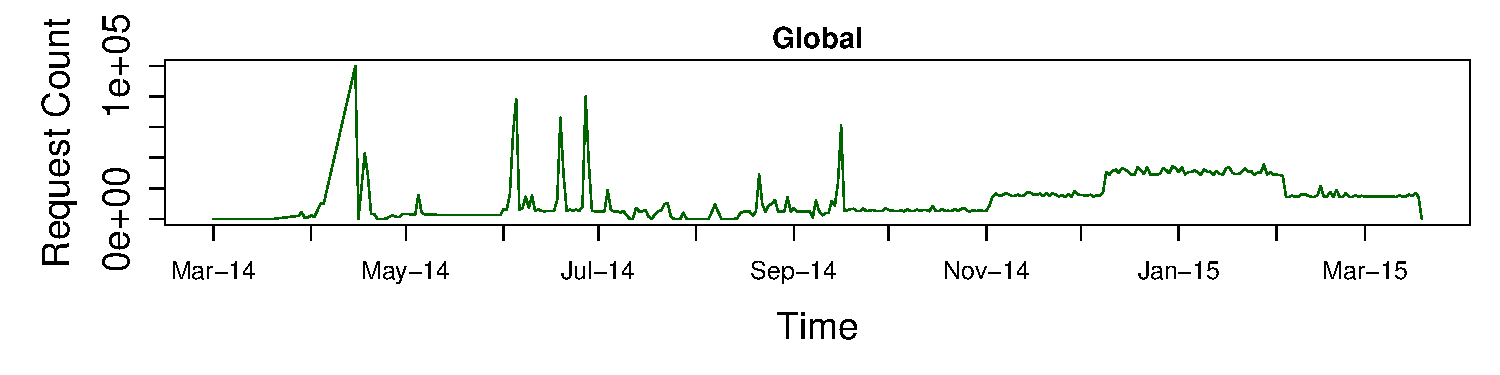
\includegraphics[width=0.9\textwidth]{imgs/ts-global-requests.pdf}
\end{figure}

%/home/rowem/Documents/Git/cmp-analysis/plotting-scripts/plots/

\begin{figure}[h!]
\caption{\csentence{Number of URL requests made per broadband ISP filter}}
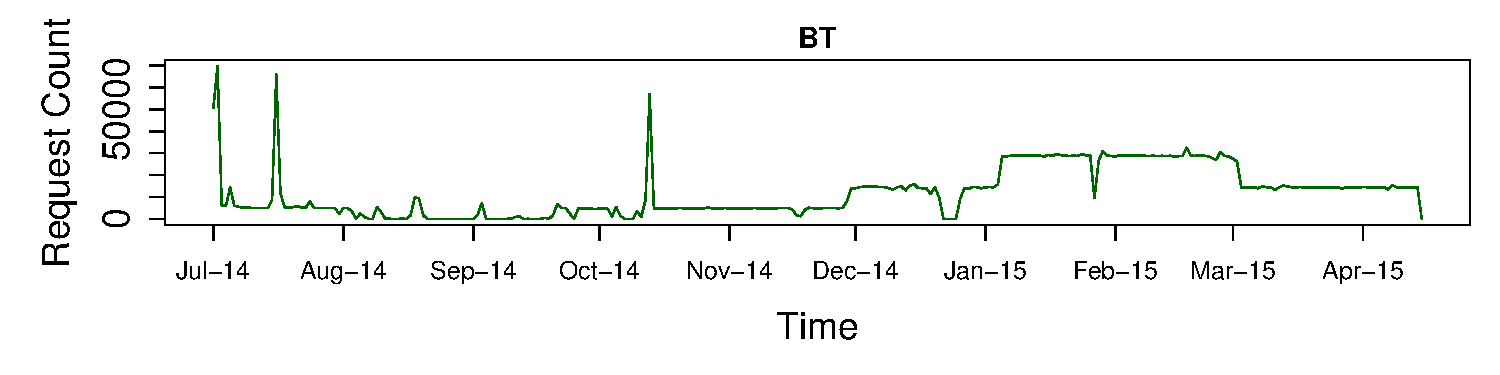
\includegraphics[width=0.49\textwidth]{imgs/BT-ts-requests.pdf}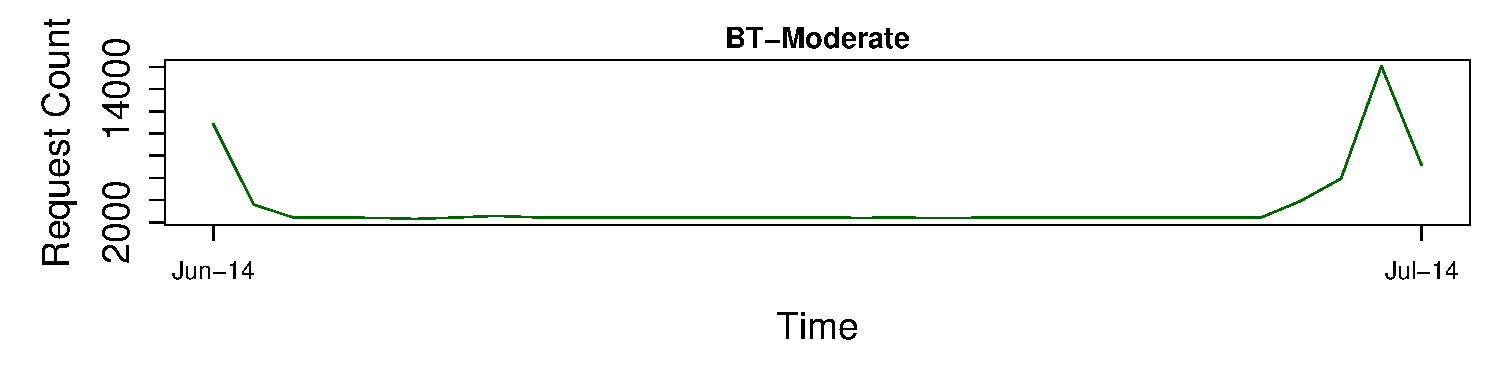
\includegraphics[width=0.49\textwidth]{imgs/BT-Moderate-ts-requests.pdf}
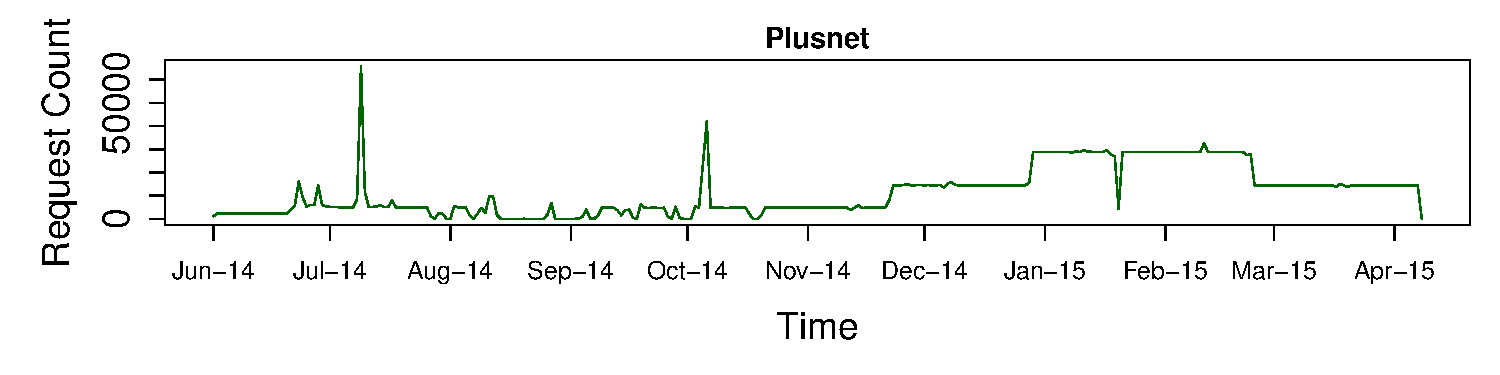
\includegraphics[width=0.49\textwidth]{imgs/Plusnet-ts-requests.pdf}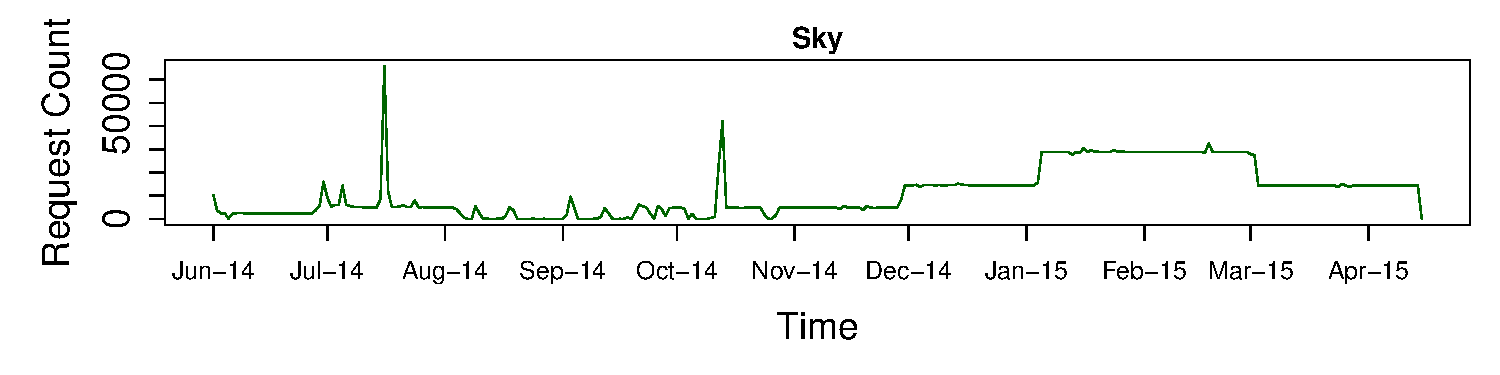
\includegraphics[width=0.49\textwidth]{imgs/Sky-ts-requests.pdf}
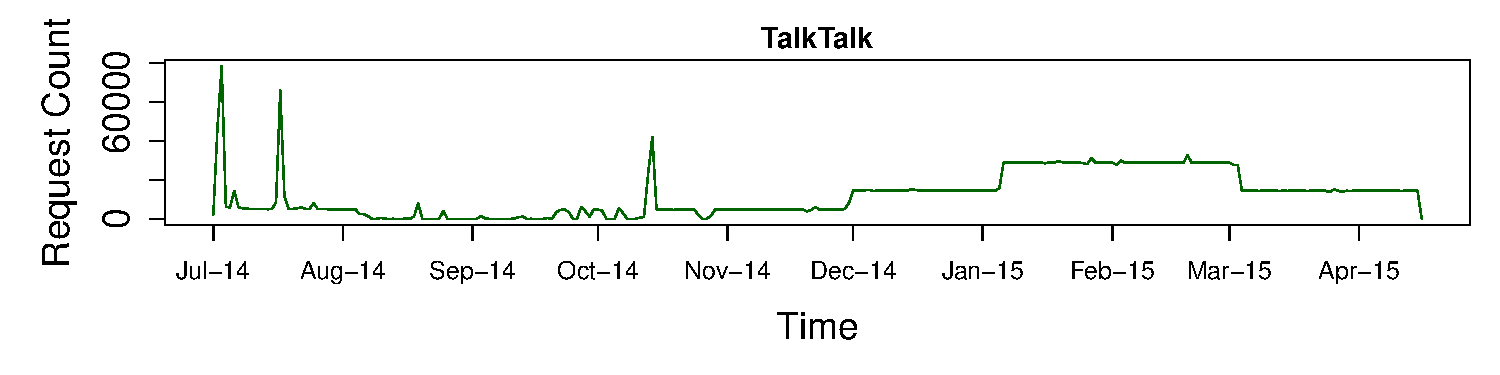
\includegraphics[width=0.49\textwidth]{imgs/TalkTalk-ts-requests.pdf}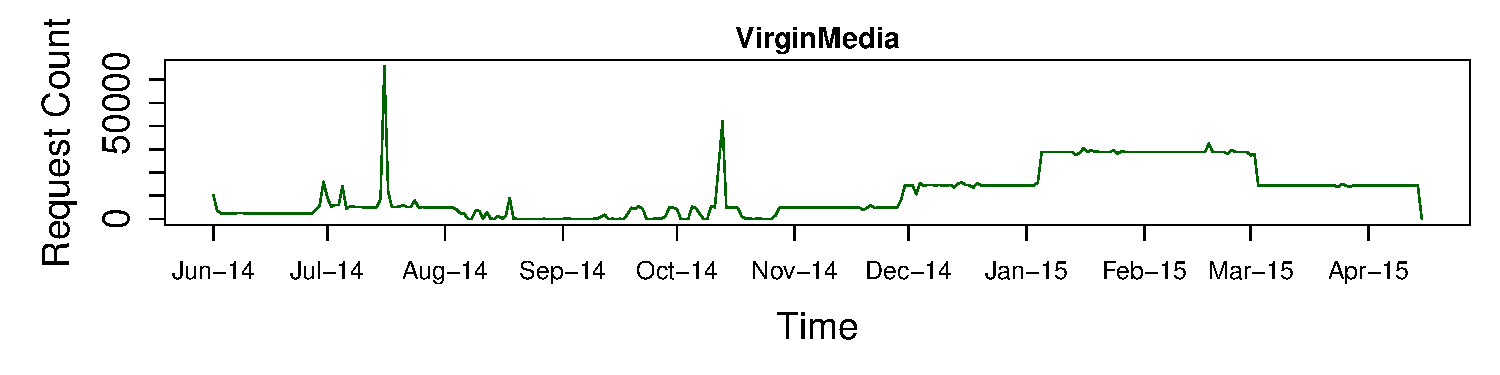
\includegraphics[width=0.49\textwidth]{imgs/VirginMedia-ts-requests.pdf}
\label{fig:broadband-requests}
\end{figure}

\begin{figure}[h!]
\caption{\csentence{Number of URL requests made per mobile ISP filter}}
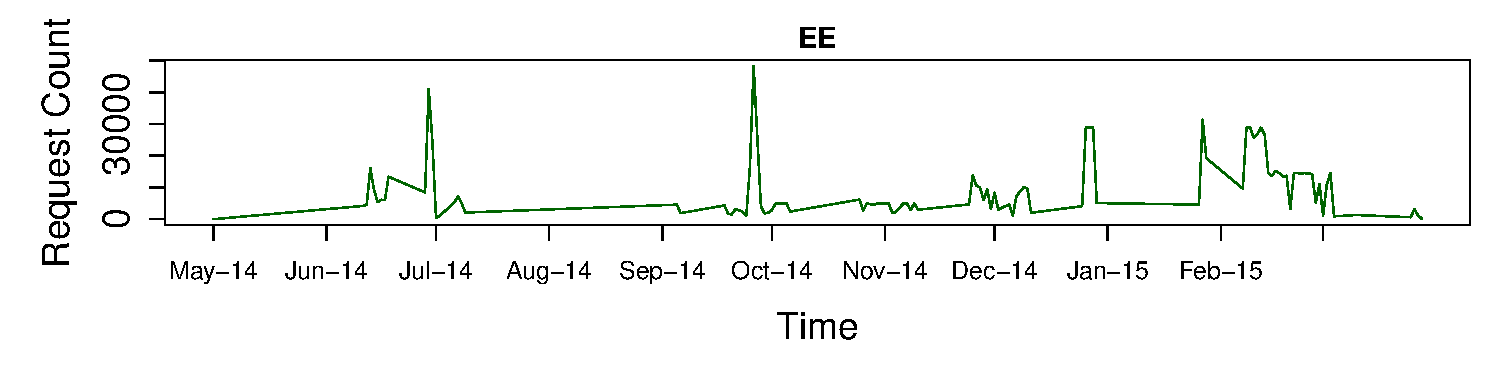
\includegraphics[width=0.49\textwidth]{imgs/EE-ts-requests.pdf}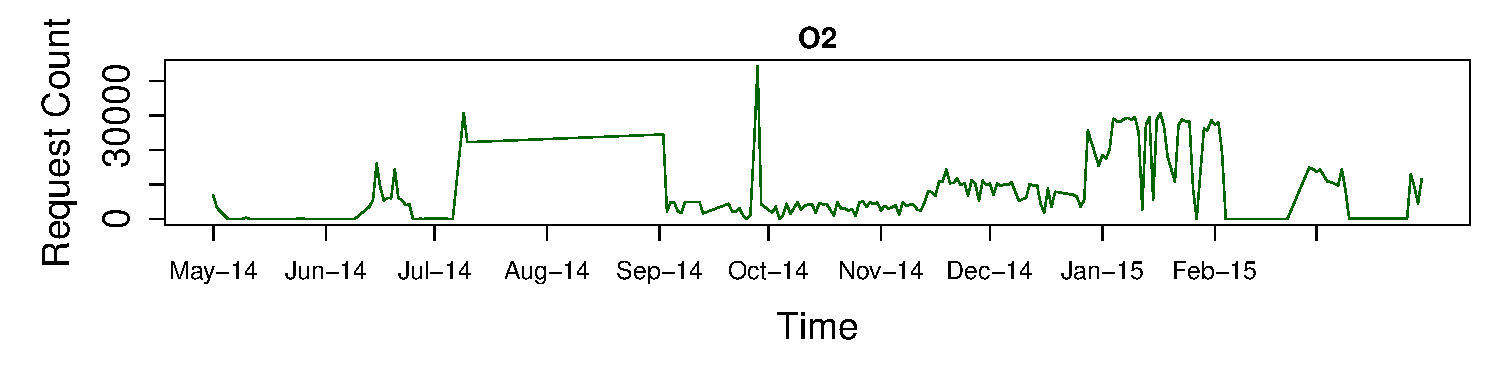
\includegraphics[width=0.49\textwidth]{imgs/O2-ts-requests.pdf}
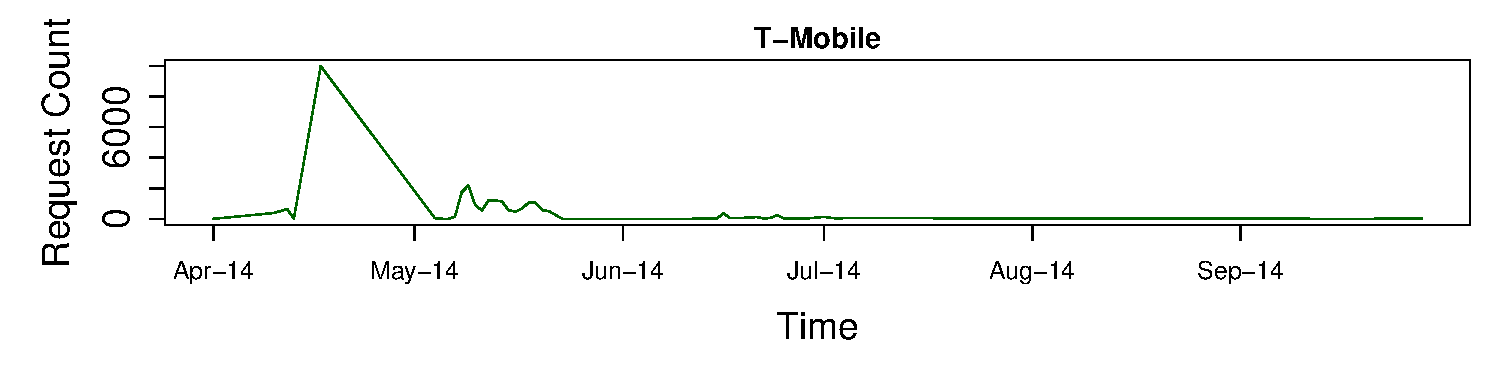
\includegraphics[width=0.49\textwidth]{imgs/T-Mobile-ts-requests.pdf}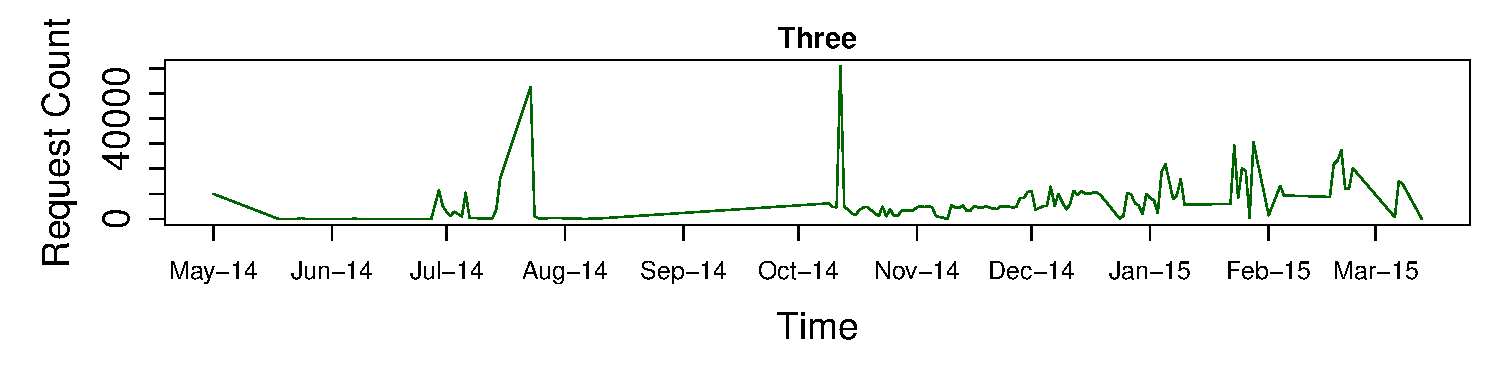
\includegraphics[width=0.49\textwidth]{imgs/Three-ts-requests.pdf}
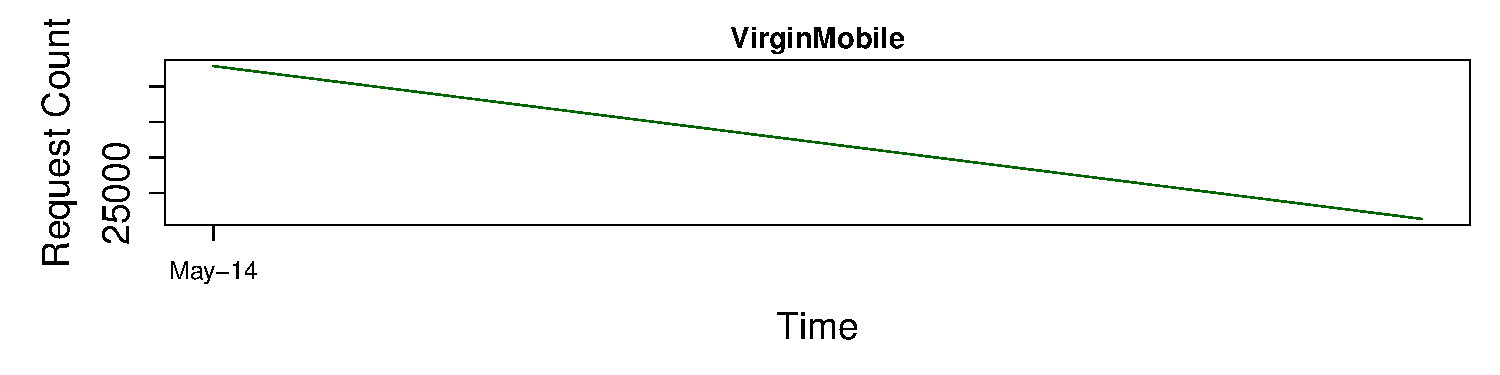
\includegraphics[width=0.49\textwidth]{imgs/VirginMobile-ts-requests.pdf}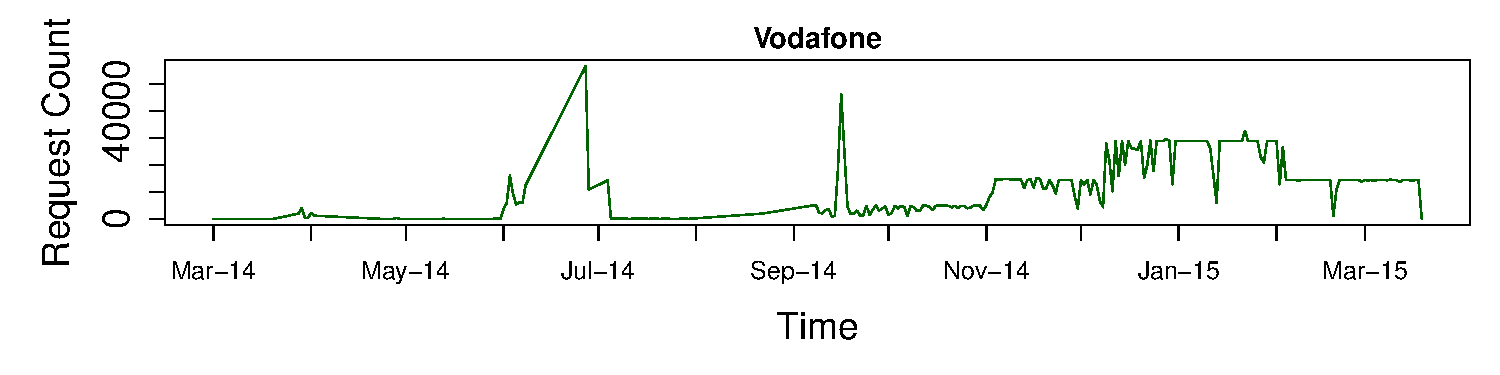
\includegraphics[width=0.49\textwidth]{imgs/Vodafone-ts-requests.pdf}
\label{fig:broadband-requests}
\end{figure}

Mobile ISP findings:
-Dropping VirginMobile from the analysis as there was a problem with the data
-Can only analyse T-Mobile up to the end of September 2014

Dropped filters:
-BT-Moderate
-VirginMobile
-T-Mobile



\clearpage
\section*{Blocked Content}

\subsection*{Blocked Domains}
-Report on distribution of domains that are blocked so far to date (ignoring changes)

\begin{figure}[h!]
\caption{\csentence{Distributions of blocked domains for broadband ISPs} This presents which domains each ISP has blocked and the frequency distribution of those domains.}
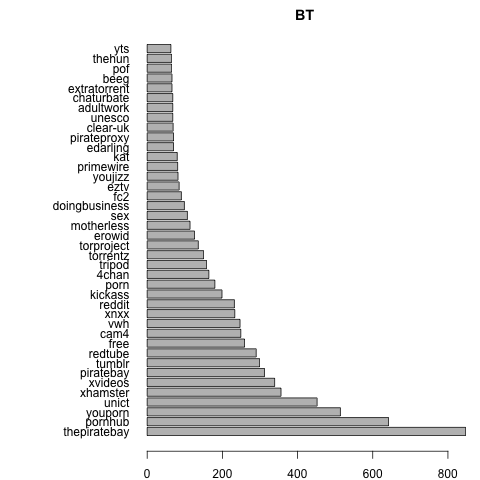
\includegraphics[width=0.49\textwidth]{imgs/BT-blocked-pages-to-date}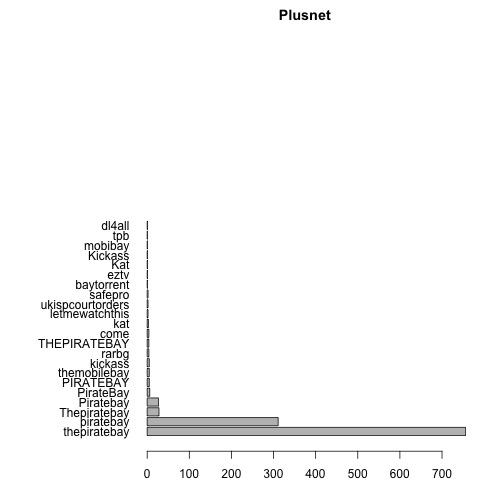
\includegraphics[width=0.49\textwidth]{imgs/Plusnet-blocked-pages-to-date}
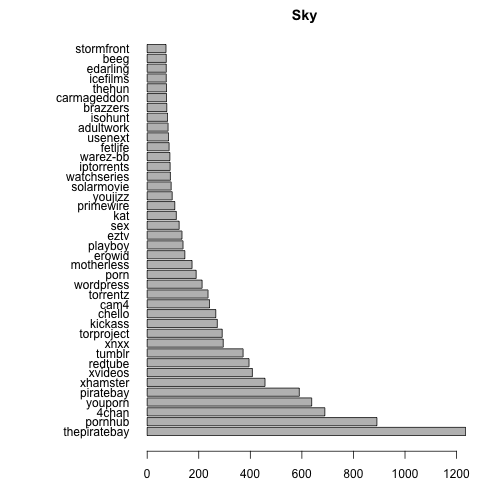
\includegraphics[width=0.49\textwidth]{imgs/Sky-blocked-pages-to-date.png}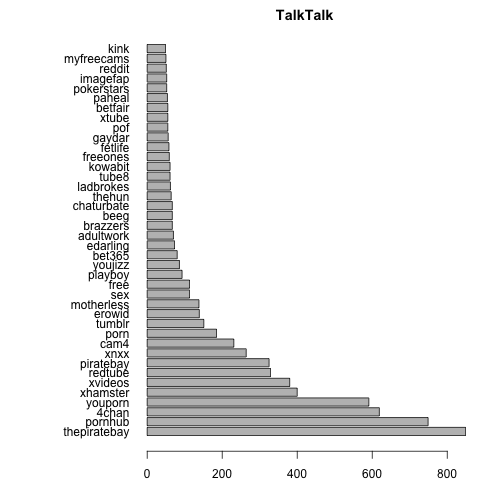
\includegraphics[width=0.49\textwidth]{imgs/TalkTalk-blocked-pages-to-date}
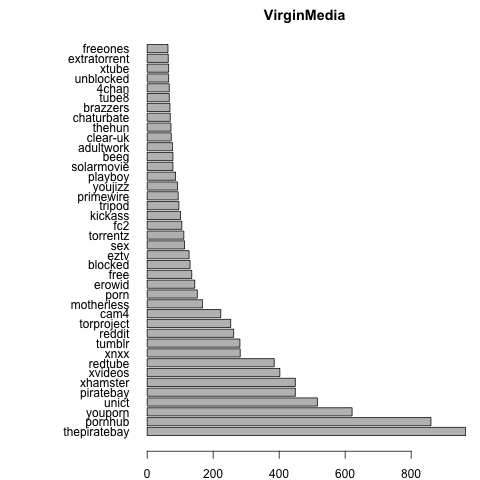
\includegraphics[width=0.49\textwidth]{imgs/VirginMedia-blocked-pages-to-date}
\label{fig:broadband-blocked-domains}
\end{figure}


\begin{figure}[h!]
\caption{\csentence{Distributions of blocked domains for mobile ISPs} This presents which domains each ISP has blocked and the frequency distribution of those domains.}
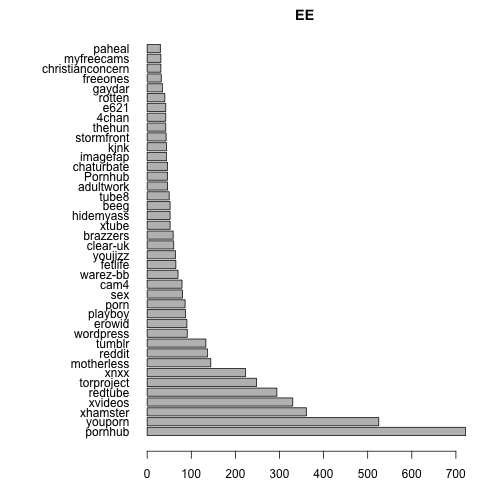
\includegraphics[width=0.49\textwidth]{imgs/EE-blocked-pages-to-date}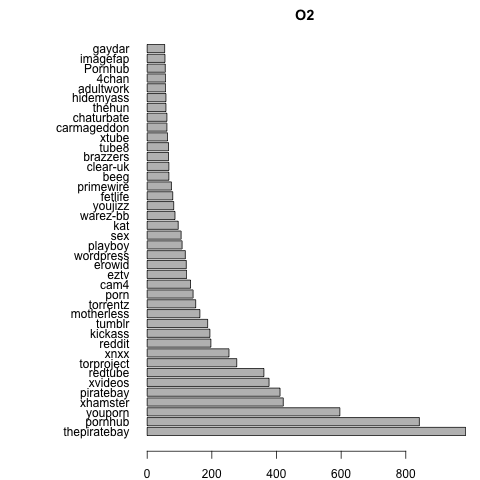
\includegraphics[width=0.49\textwidth]{imgs/O2-blocked-pages-to-date}
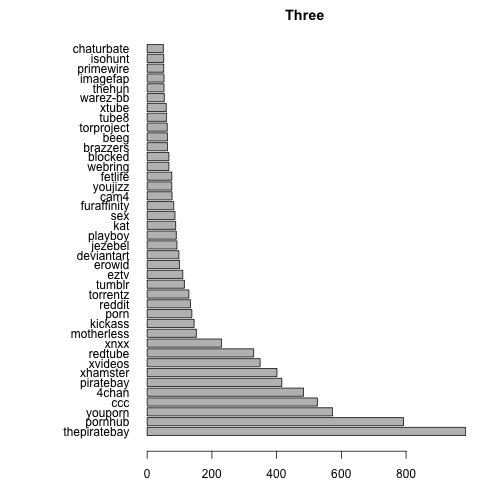
\includegraphics[width=0.49\textwidth]{imgs/Three-blocked-pages-to-date.png}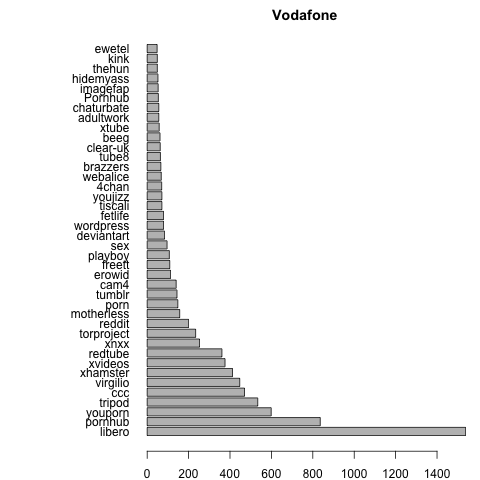
\includegraphics[width=0.49\textwidth]{imgs/Vodafone-blocked-pages-to-date}
\label{fig:mobile-blocked-domains}
\end{figure}


To do:
-Add analysis of wordpress, tumblr, reddit, and livejournal sites

Wordpress Examples:
-URL: http://beeractivist.wordpress.com | Submitted: 2014-11-30 21:13:51 | NetworkName: TalkTalk | Status: blocked
-URL: http://tantracore.wordpress.com | Submitted: 2014-11-30 22:13:28 | NetworkName: Sky | Status: blocked
-URL: http://garsai.wordpress.com | Submitted: 2014-11-30 23:02:46 | NetworkName: TalkTalk | Status: blocked
-URL: http://toysoldier.wordpress.com | Submitted: 2014-07-03 15:03:15 | NetworkName: O2 | Status: blocked
--This site is a support site for men who have been abused (also blocked by Sky)
-URL: http://www.heyartist.wordpress.com | Submitted: 2014-11-30 20:56:34 | NetworkName: Sky | Status: blocked
--Site promoting art as a support mechanism for enhancing wellbeing

Tumblr Examples:
-URL: http://atlasofprejudice.tumblr.com | Submitted: 2014-05-14 01:12:57 | NetworkName: TalkTalk Strict | Status: blocked
--Showing examples of maps that demonstrate the prejudices that countries have
-URL: http://azurelunatic.tumblr.com/post/18654147576/ive-been-forced-to-explain-homosexuality-to-my | Submitted: 2014-05-27 21:27:00 | NetworkName: Vodafone | Status: blocked
--Example of blocking a site as it contains an explanation of why someone is gay (potential prejudice here). Also blocked by O2, TalkTalk, and BT
-URL: http://thusly.tumblr.com | Submitted: 2014-07-02 13:08:44 | NetworkName: EE | Status: blocked
--Also blocked by BT, Sky, O2, Vodafone
-URL: http://tldrwikipedia.tumblr.com | Submitted: 2014-05-14 01:13:11 | NetworkName: TalkTalk | Status: blocked
-URL: http://notalkingplz.tumblr.com | Submitted: 2014-07-02 14:22:20 | NetworkName: O2 | Status: blocked
--Also blocked on: Sky, Vodafone, EE


Reddit Examples:
-Largely blocking http://www.reddit.com/r/nsfw, http://www.reddit.com/r/nsfl, and http://reddit.com/r/porn, all of which are sub-reddits containing adult content
-URL: http://www.reddit.cm | Submitted: 2014-07-02 10:40:30 | NetworkName: Sky | Status: blocked
-URL: http://reddit.com/r/creepypms | Submitted: 2014-07-05 20:10:31 | NetworkName: EE | Status: blocked
--Subreddit sharing creepy private messages that people have received. Not necessarily adult content, and definitely not pornography.


Livejournal:
-All appear to the sites of Russian sites (e.g. http://limonov-eduard.livejournal.com/)

-URL: http://community.livejournal.com/asi/ | Submitted: 2014-11-30 21:11:19 | NetworkName: Sky | Status: blocked
--Anorexia and self-harm support community site. Contains posts from people explaining their afflictions and getting support from other people.

-URL: http://beer-retard.livejournal.com | Submitted: 2014-11-30 21:13:51 | NetworkName: TalkTalk | Status: blocked
--Blocked due to discussing/containing information about alcohol/beer?

-URL: http://urban-decay.livejournal.com | Submitted: 2014-11-30 21:14:59 | NetworkName: Sky | Status: blocked
--Also blocked by Three and O2

-URL: http://ercasse-ainince.livejournal.com/30230.html | Submitted: 2014-11-30 20:51:44 | NetworkName: Sky | Status: blocked
--Article about films that have been out for a long time

-Largely blocking pornography live journal pages too



\subsection*{Blocked Site Categories}
-Report on the distribution of categories of sites that are blocked
--Explain the categorisation system used, and the various levels of categories
--What is the coverage of URLs in the DMOZ categorisation system? Report on the \% covered in the system

Given the DMOZ categorisation system and the use of ODP categories, we can use the hierarchy of the category taxonomy to only focus up to a specific depth; thereby restricting the categories to only depth of $d$.

\begin{figure}[h!]
\caption{\csentence{Distributions of blocked level-4 categories for broadband ISPs.}}
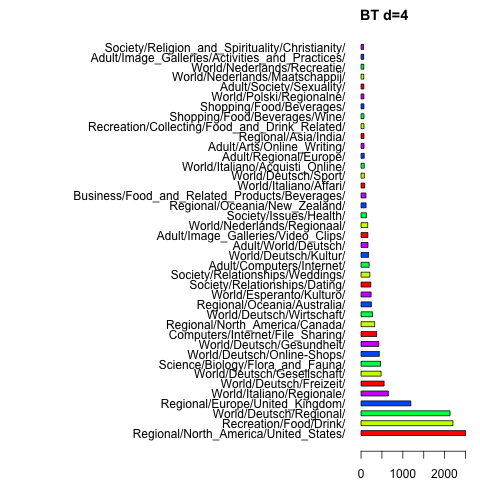
\includegraphics[width=0.49\textwidth]{imgs/BT-d-4-blocked-categories-to-date.png}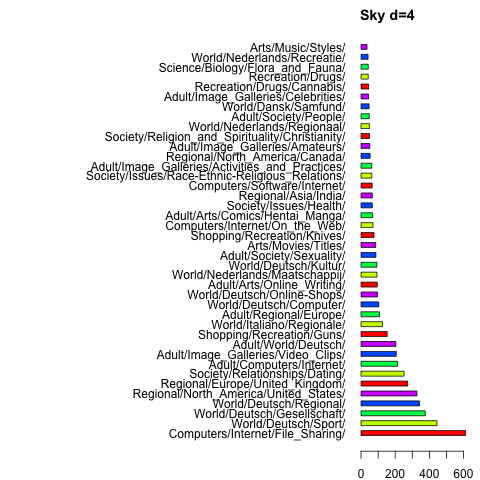
\includegraphics[width=0.49\textwidth]{imgs/Sky-d-4-blocked-categories-to-date.png}
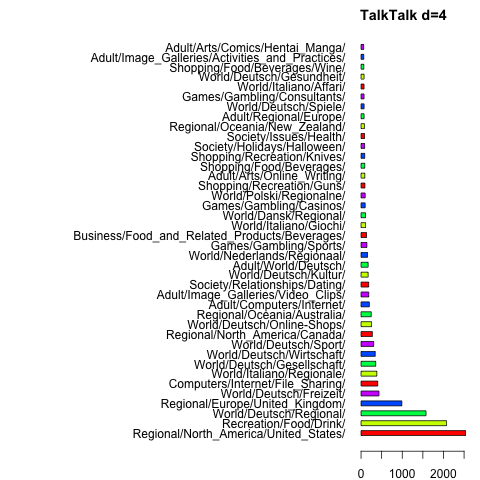
\includegraphics[width=0.49\textwidth]{imgs/TalkTalk-d-4-blocked-categories-to-date.png}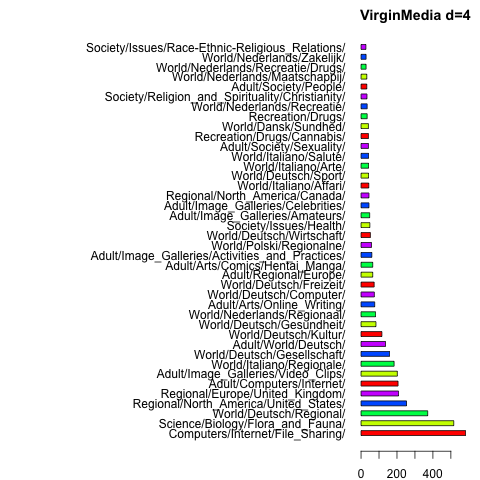
\includegraphics[width=0.49\textwidth]{imgs//VirginMedia-d-4-blocked-categories-to-date.png}
\label{fig:broadband-blocked-categories}
\end{figure}

-Not showing Plusnet as it blocks file-sharing category sites

\begin{figure}[h!]
\caption{\csentence{Distributions of blocked level-4 categories for mobile ISPs.}}
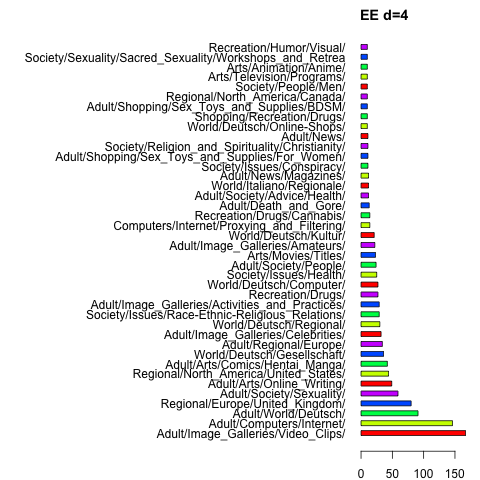
\includegraphics[width=0.49\textwidth]{imgs/EE-d-4-blocked-categories-to-date.png}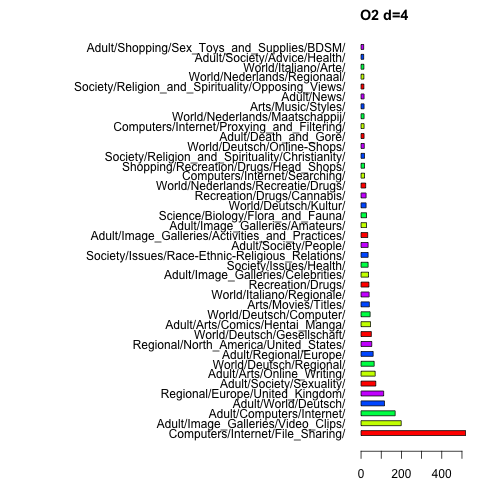
\includegraphics[width=0.49\textwidth]{imgs/O2-d-4-blocked-categories-to-date.png}
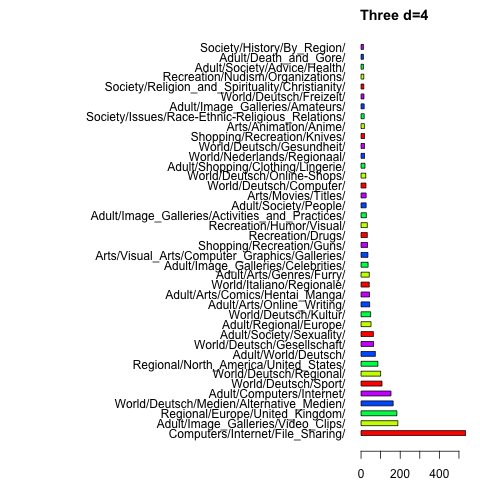
\includegraphics[width=0.49\textwidth]{imgs/Three-d-4-blocked-categories-to-date.png}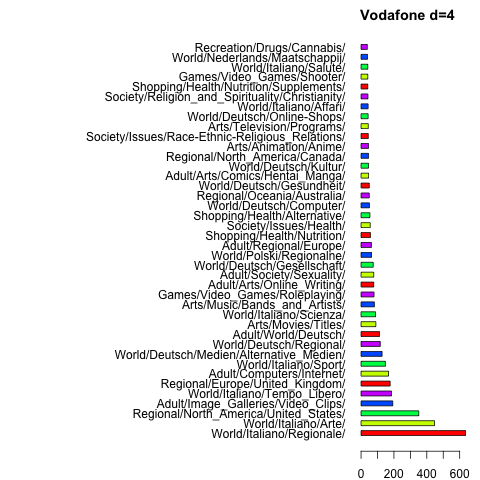
\includegraphics[width=0.49\textwidth]{imgs/Vodafone-d-4-blocked-categories-to-date.png}
\label{fig:broadband-blocked-categories}
\end{figure}


%%%%%% Section
\clearpage
\section*{Gauging Filter Accuracy}
-Report on reverse engineering the accuracy of the filters
--Need to consider how to collect certain porrnographic examples here and push them to the blocked.org.uk queue
--Report on the class balance between blocked vs not-blocked content
--Can only consider URLs within the system?
--Do the findings suggest a certain problem with the mechanisms used to classify urls?

\subsection*{Pseudo-Classifiers for ISP Filters}
-Induce a pseudo-classifier for each ISP filter setting:
--Specify which categories of content should be blocked by certain filter
--Add table to explain this
--Coded blocked topics into DMOZ categories to identify what the pseudo classifier should block. 
--Our approach is to always go as conservative as possible: i.e. if unsure about whether a category should be blocked, then block it.
--Remove file-sharing for now, as this is assessed on a case-by-case basis and with court orders
---I.e. blocking all of Computers: Software: Internet: File Sharing would lead to studies on file-sharing being blocked
--Hence: block everything under Adult
--Also block everything under Computers/Hacking

-BT: should block...
--pornography (Adult/Image Galleries + Adult/Video Clips)
--obscene and tasteless (Adult/Death and Gore)
--hate and self-harm (no DMOZ category)
--drugs (Recreation/Drugs)
--alcohol (Recreation/Food/Drink/Drinking + Health/Specific Substances/Alcoholic Beverages)
--tobacco (Shopping/Tobacco + Recreation/Tobacco)
--dating (Society/Relationships/Dating, Society/Relationships/Cyber\_Relationships)

-Sky: should block...
--malware sites (Computers/Security/Malicious\_Software/Spyware\_and\_Adware)
--cyber-bullying (no cat on this, generally there are advice pages though)
--pornography (Adult)
--suicide and self-harm (no cat)
--drugs (Recreation/Drugs)
--dating (Society/Relationships/Dating)
--social networking (Computers/Internet/On\_the\_Web/Online\_Communities/Social\_Networking, Kids\_and\_Teens/People\_and\_Society/Online Communities)
--online gaming (Games/Online)

-TalkTalk: should block...
--dating (Society/Relationships/Dating)
--drugs (Recreation/Drugs)
--alcohol (Recreation/Food/Drink/Drinking + Health/Specific Substances/Alcoholic Beverages)
--tobacco (Shopping/Tobacco + Recreation/Tobacco)
--File Sharing Sites (Computers/Software/Internet/Clients/File Sharing)
--Gambling (Gamling)
--online gaming (Games)
--Pornography (Adult)
--social networking (Computers/Internet/On\_the\_Web/Online\_Communities/Social\_Networking, Kids\_and\_Teens/People\_and\_Society/Online Communities)
--Suicide and Self-Harm (no cat)
--Weapons and Violence (Adult)

VirginMedia: should block...
--Crime, Violence, and Hate: (Adult)
--Drugs (Recreation/Drugs/Cannabis + Recreation/Drugs/Psychedelics)
--File Sharing Sites (Computers/Software/Internet/Clients/File Sharing)
--Pornography (Adult)
--Suicide and Self-harm (no category for this in DMOZ)


-EE, O2, and Three: should block...

--18 works are for adults and can contain strong issues such as: very strong violence, frequent strong language (e.g. 'f***') and / or very strong language (e.g. ‘c***’), strong portrayals of sexual activity, scenes of sexual violence, strong horror, strong blood and gore, real sex (in some circumstances), discriminatory language and behaviour

-Vodafone: should block...
--Our content control prevents access to 18-rated content on Vodafone live! (mobile internet) and blocks access to 18-rated websites, un-moderated chat rooms and listed child abuse sites.



From the DMOZ web site: 
Generally the Adult category includes sites whose dominant theme is either:
-To appeal to the prurient interest in sex without any serious literary, artistic, political, or scientific value
-The depiction or description of nudity, including sexual or excretory activities or organs in a lascivious way
-The depiction or description of sexually explicit conduct in a lascivious way (e.g. for entertainment purposes)



\subsection*{Judging Filter Accuracy}

Explain gauging filter accuracy using existing measures from classification literature.
-Parallelisation of the accuracy measurement
-Explain the role of Spark in this to distribute the work load
-Explain the location of the code and how to run this
-Explain how we calculate accuracy based on which requests were blocked and which were not blocked - we have to do this as a URL can go from blocked to unblocked and vice-versa
--Question: how often is a given URL periodically tested for a block?


\subsubsection*{General Accuracy}

% Original results without assessing for polysemic categories
\begin{table}[h!]
\caption{Accuracy levels of ISP and Mobile Providers' Web Filters derived using the DMOZ categories that should have been blocked by each filter and the categories of URLs that were actually blocked.}
  \begin{tabular}{ l c c c c c c}
    \hline
     & Precision & Recall & FPR & MCC & F1 \\
    \hline
	BT & 0.032 & 0.613 & 0.012 & 0.138 & 0.061 \\
    Sky & 0.088 & 0.370 & 0.003 & 0.179 & 0.142 \\
    TalkTalk & 0.078  & 0.073 & 0.009 & 0.066 & 0.075 \\
	VirginMedia & 0.050 & 0.508 & 0.003 & 0.159 & 0.091 \\
	\hline    
	EE & 0.189 & 0.635 & 0.002 & 0.346 & 0.291 \\
	O2 & 0.136 & 0.697 & 0.002 & 0.307 & 0.227 \\
	Three & 0.108 & 0.631 & 0.004 & 0.260 & 0.185 \\
	Vodafone & 0.044 & 0.564 & 0.004 & 0.156 & 0.081 \\
    \hline
  \end{tabular}
\end{table}

% Updated results (21st May 2015). Shows large degradation in accuracy. After altering category checking procedure
%BT: tp = 634.0 | tn = 1543183.0 | fp = 19168.0 | fn = 400.0 | prec = 0.032 | rec = 0.613 | FPR = 0.012 | mcc = 0.138 | F1 = 0.061
%Sky: tp = 526.0 | tn = 1566677.0 | fp = 5442.0 | fn = 895.0 | prec = 0.088 | rec = 0.370 | FPR = 0.003 | mcc = 0.179 | F1 = 0.142
%TalkTalk: tp = 1218.0 | tn = 1542758.0 | fp = 14409.0 | fn = 15514.0 | prec = 0.078  | rec = 0.073 | FPR = 0.009 | mcc = 0.066 | F1 = 0.075
%VirginMedia: tp = 266.0 | tn = 1568395.0 | fp = 5036.0 | fn = 258.0 | prec = 0.0502  | rec = 0.508 | FPR = 0.003 | mcc = 0.159 | F1 = 0.091
%EE: tp = 219.0 | tn = 472432.0 | fp = 939.0 | fn = 126.0 | prec = 0.189 | rec = 0.635 | FPR = 0.002 | mcc = 0.346 | F1 = 0.291
%O2: tp = 230.0 | tn = 876122.0 | fp = 1462.0 | fn = 100.0 | prec = 0.136 | rec = 0.697 | FPR = 0.002 | mcc = 0.307 | F1 = 0.227
%Three: tp = 236.0 | tn = 491864.0 | fp = 1941.0 | fn = 138.0 | prec = 0.108 | rec = 0.631 | FPR = 0.004 | mcc = 0.260 | F1 = 0.185
%Vodafone: tp = 254.0 | tn = 1482343.0 | fp = 5560.0 | fn = 196.0 | prec = 0.044 | rec = 0.564 | FPR = 0.004 | mcc = 0.156 | F1 = 0.081

\begin{table}[h!]
\caption{Accuracy levels after filtering out sites from the World category subtree.}
  \begin{tabular}{ l c c c c c c}
    \hline
     & Precision & Recall & FPR & MCC & F1 \\
    \hline
	BT & 0.066 & 0.612 & 0.010 & 0.198 & 0.119 \\
    Sky & 0.163 & 0.372 & 0.003 & 0.245 & 0.227 \\
    TalkTalk & 0.145 & 0.072 & 0.008 & 0.091 & 0.097 \\
	VirginMedia & 0.112 & 0.512 & 0.002 & 0.239 & 0.184 \\
	\hline    
	EE & 0.281 & 0.637 & 0.002 & 0.422 & 0.390 \\
	O2 & 0.218 & 0.699 & 0.002 & 0.390 & 0.333 \\
	Three & 0.184 & 0.633 & 0.004 & 0.340 & 0.285 \\
	Vodafone & 0.083 & 0.568 & 0.003 & 0.216 & 0.144 \\
    \hline
  \end{tabular}
\end{table}


% Updated results (29th May 2015). After altering the world category filter
%BT: tp = 627.0 | tn = 867824.0 | fp = 8919.0 | fn = 398.0 | prec = 0.066 | rec = 0.612 | FPR = 0.010 | mcc = 0.198 | F1 = 0.119
%Sky: tp = 520.0 | tn = 879512.0 | fp = 2663.0 | fn = 876.0 | prec = 0.163 | rec = 0.372 | FPR = 0.003 | mcc = 0.245 | F1 = 0.227
%TalkTalk: tp = 1201.0 | tn = 860146.0 | fp = 7065.0 | fn = 15375.0 | prec = 0.145 | rec = 0.072 | FPR = 0.008 | mcc = 0.091 | F1 = 0.097
%VirginMedia: tp = 266.0 | tn = 881118.0 | fp = 2105.0 | fn = 254.0 | prec = 0.112 | rec = 0.512 | FPR = 0.002 | mcc = 0.239 | F1 = 0.184
%EE: tp = 219.0 | tn = 269566.0 | fp = 561.0 | fn = 125.0 | prec = 0.281 | rec = 0.637 | FPR = 0.002 | mcc = 0.422 | F1 = 0.390
%O2: tp = 230.0 | tn = 494277.0 | fp = 823.0 | fn = 99.0 | prec = 0.218 | rec = 0.699 | FPR = 0.002 | mcc = 0.390 | F1 = 0.333
%Three: tp = 236.0 | tn = 280598.0 | fp = 1046.0 | fn = 137.0 | prec = 0.184 | rec = 0.633 | FPR = 0.004 | mcc = 0.340 | F1 = 0.285
%Vodafone: tp = 254.0 | tn = 832797.0 | fp = 2819.0 | fn = 193.0 | prec = 0.083 | rec = 0.568 | FPR = 0.003 | mcc = 0.216 | F1 = 0.144

\begin{table}[h!]
\caption{Accuracy levels after filtering out sites from the World category subtree and controlling for breweries and other alcohol related sites.}
  \begin{tabular}{ l c c c c c c}
    \hline
     & Precision & Recall & FPR & MCC & F1 \\
    \hline
	BT & 0.335 & 0.726 & 0.007 & 0.490 & 0.459 \\
    Sky & 0.163 & 0.372 & 0.003 & 0.245 & 0.227 \\
    TalkTalk & 0.422 & 0.176 & 0.006 & 0.262 & 0.248 \\
	VirginMedia & 0.112 & 0.512 & 0.002 & 0.239 & 0.184 \\
	\hline    
	EE & 0.281 & 0.637 & 0.002 & 0.422 & 0.390 \\
	O2 & 0.218 & 0.699 & 0.002 & 0.390 & 0.333 \\
	Three & 0.184 & 0.633 & 0.004 & 0.340 & 0.285 \\
	Vodafone & 0.083 & 0.568 & 0.003 & 0.216 & 0.144 \\
    \hline
  \end{tabular}
\end{table}

% Updated results (29th May 2015). After fixing the alcohol sites
%BT: tp = 3202.0 | tn = 867015.0 | fp = 6344.0 | fn = 1207.0 | prec = 0.335 | rec = 0.726 | FPR = 0.007 | mcc = 0.490 | F1 = 0.459
%Sky: tp = 520.0 | tn = 879512.0 | fp = 2663.0 | fn = 876.0 | prec = 0.163 | rec = 0.372 | FPR = 0.003 | mcc = 0.245 | F1 = 0.227
%TalkTalk: tp = 3485.0 | tn = 859202.0 | fp = 4781.0 | fn = 16319.0 | prec = 0.422 | rec = 0.176 | FPR = 0.006 | mcc = 0.262 | F1 = 0.248
%VirginMedia: tp = 266.0 | tn = 881118.0 | fp = 2105.0 | fn = 254.0 | prec = 0.112 | rec = 0.512 | FPR = 0.002 | mcc = 0.239 | F1 = 0.184
%EE: tp = 219.0 | tn = 269566.0 | fp = 561.0 | fn = 125.0 | prec = 0.281 | rec = 0.637 | FPR = 0.002 | mcc = 0.422 | F1 = 0.390
%O2: tp = 230.0 | tn = 494277.0 | fp = 823.0 | fn = 99.0 | prec = 0.218 | rec = 0.699 | FPR = 0.002 | mcc = 0.390 | F1 = 0.333
%Three: tp = 236.0 | tn = 280598.0 | fp = 1046.0 | fn = 137.0 | prec = 0.184 | rec = 0.633 | FPR = 0.004 | mcc = 0.340 | F1 = 0.285
%Vodafone: tp = 254.0 | tn = 832797.0 | fp = 2819.0 | fn = 193.0 | prec = 0.083 | rec = 0.568 | FPR = 0.003 | mcc = 0.216 | F1 = 0.144



Qualitative Examples of Blocks:
-BT Block: http://www.lgbtquitsmoking.com/ (site to help people stop smoking).

BT seem to be blocking tattoo web sites too:

We have uploaded the collection of sites which are false positives and false negatives to the github repo.\footnote{\url{https://github.com/openrightsgroup/cmp-analysis/tree/master/data/output}}


\subsubsection*{Accuracy over Time}
How has accuracy evolved over time?
--Discrete time analysis of the accuracy levels - use weekly bins (Bayesian model?) Can we forecast accuracy?


\begin{figure}[h!]
\caption{\csentence{Accuracy of Broadband ISPs' filters over time}. ARIMA(0,0,5) plot of the accuracy measures: precision, recall, f-measure (F1), false positive rate (FPR), and the Matthews' Correlation Coefficient. Weeks are from the start of the ISP-specific filter logging period.}
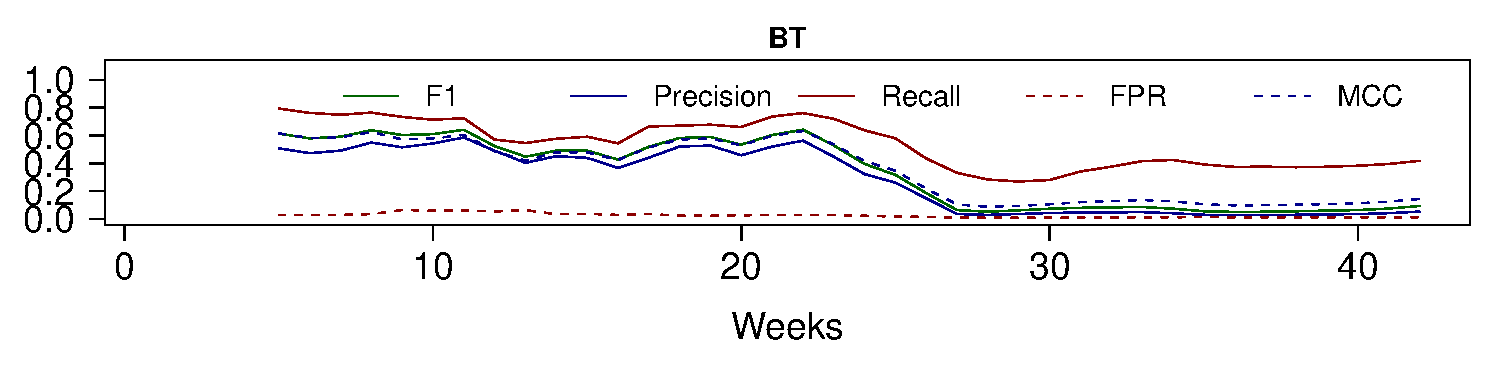
\includegraphics[width=0.9\textwidth]{imgs/BT-ts-accuracy}
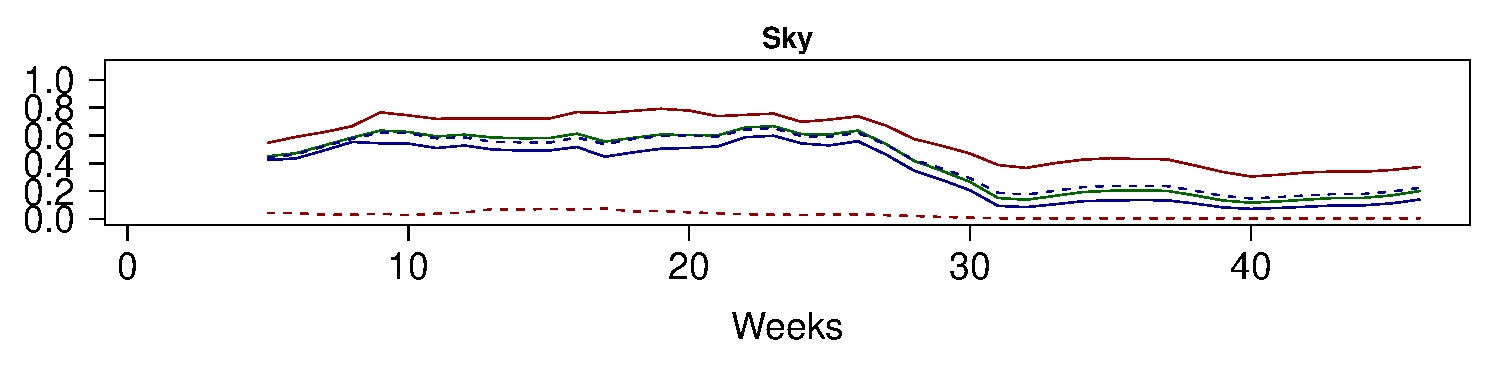
\includegraphics[width=0.9\textwidth]{imgs/Sky-ts-accuracy}
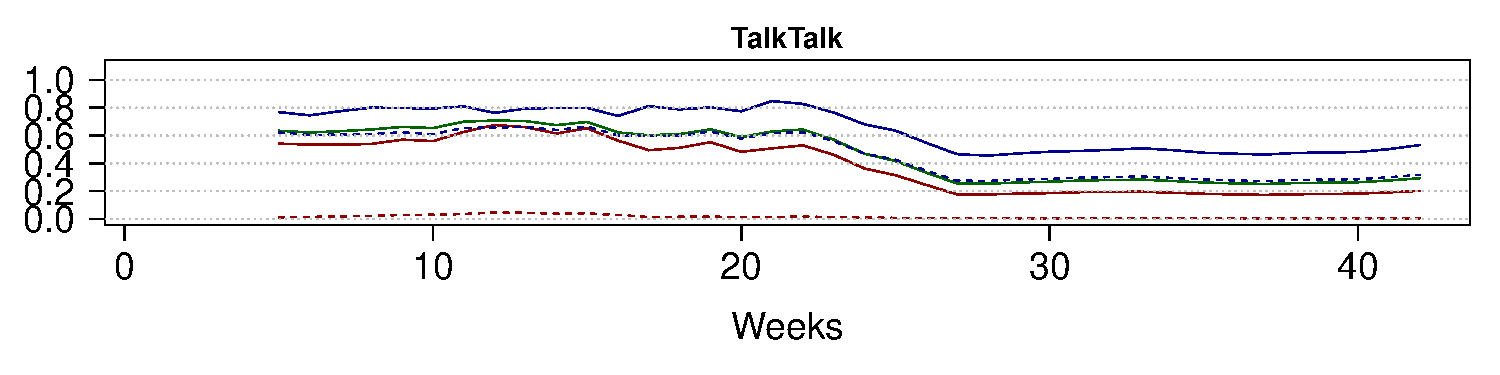
\includegraphics[width=0.9\textwidth]{imgs/TalkTalk-ts-accuracy}
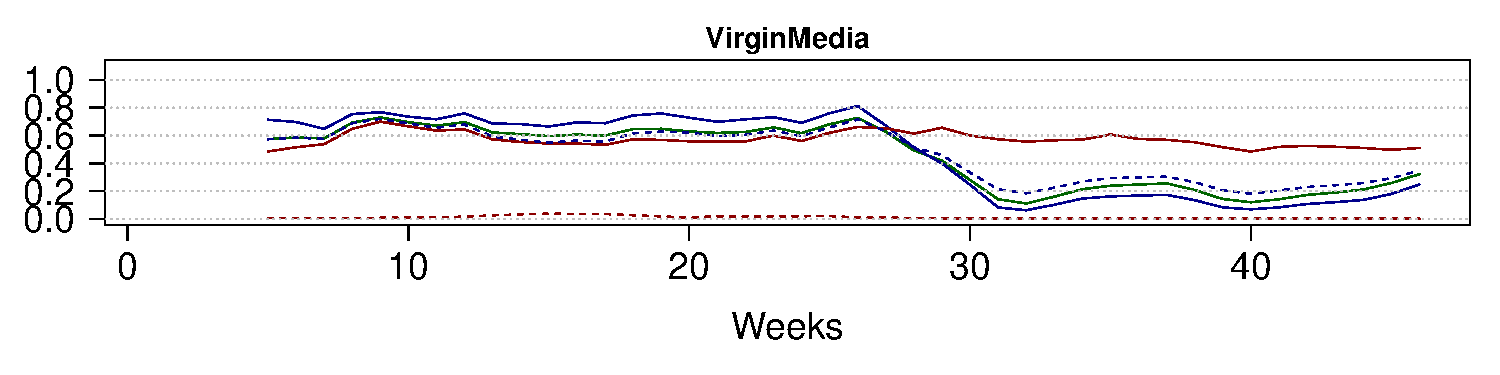
\includegraphics[width=0.9\textwidth]{imgs/VirginMedia-ts-accuracy}
\label{fig:broadband-accuracy-ts}
\end{figure}

\begin{figure}[h!]
\caption{\csentence{Accuracy of Mobile ISPs' filters over time}. ARIMA(0,0,5) plot of the accuracy measures: precision, recall, f-measure (F1), false positive rate (FPR), and the Matthews' Correlation Coefficient. Weeks are from the start of the ISP-specific filter logging period.}
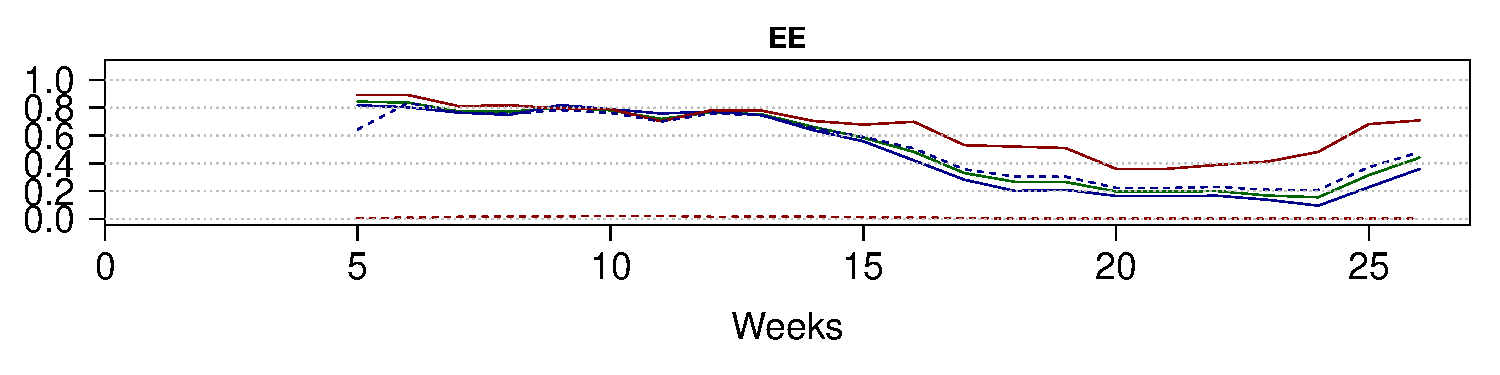
\includegraphics[width=0.9\textwidth]{imgs/EE-ts-accuracy}
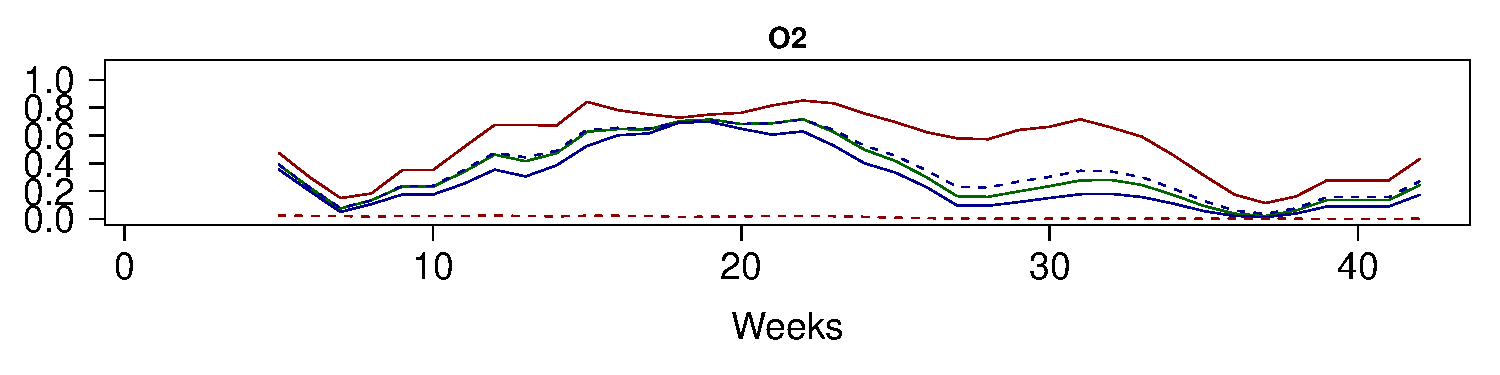
\includegraphics[width=0.9\textwidth]{imgs/O2-ts-accuracy}
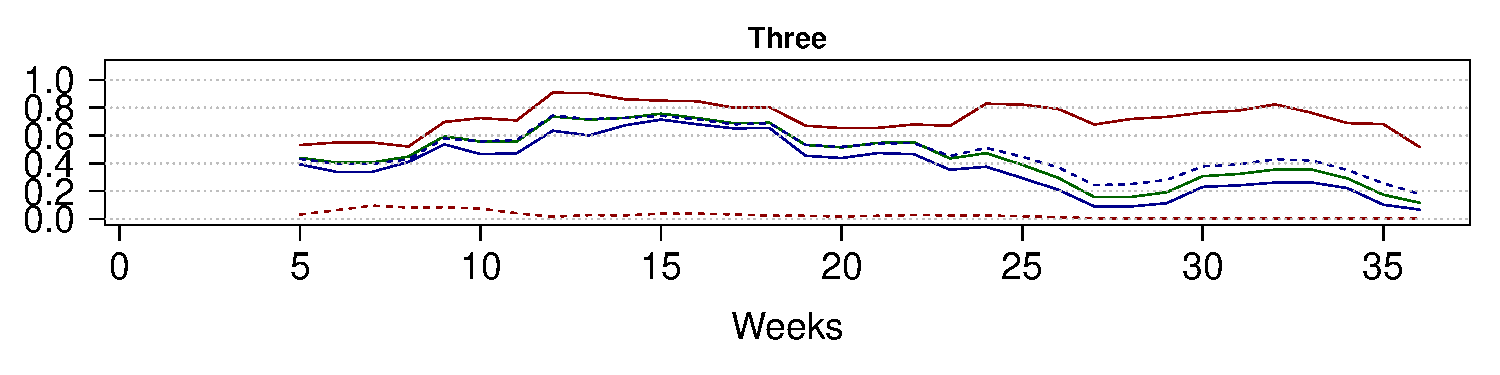
\includegraphics[width=0.9\textwidth]{imgs/Three-ts-accuracy}
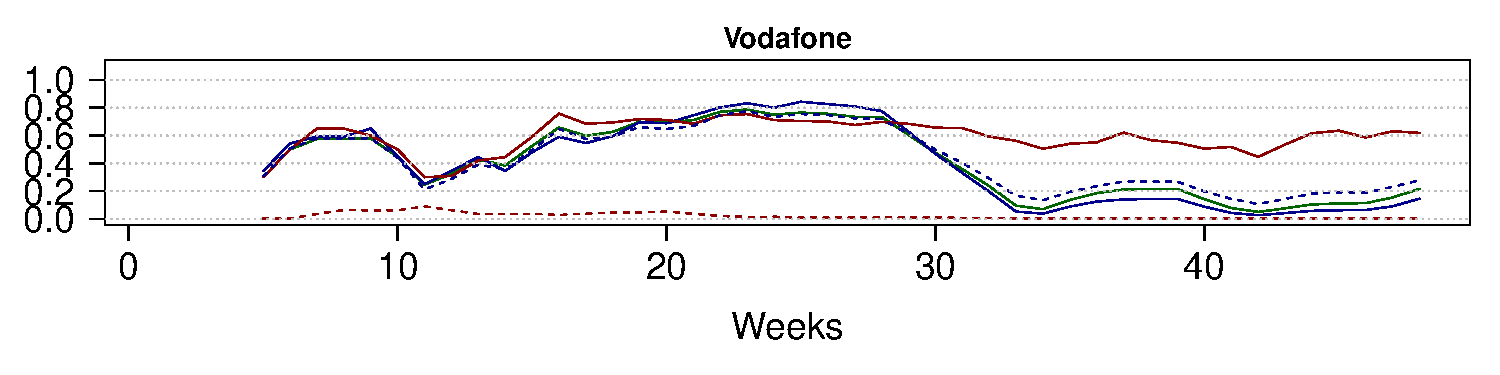
\includegraphics[width=0.9\textwidth]{imgs/Vodafone-ts-accuracy}
\label{fig:mobile-accuracy-ts}
\end{figure}
\clearpage






%%%%%% Section
\section*{Time to Correction}
-Report on how long it takes each ISP to fix their blocked content
-Show the delta distribution of each provider
--Fit a distribution to the delta-function: Poisson?

\begin{figure}[h!]
\caption{\csentence{Time to unblock ($\Delta$) distribution of each Broadband and Mobile ISP in hours}.}
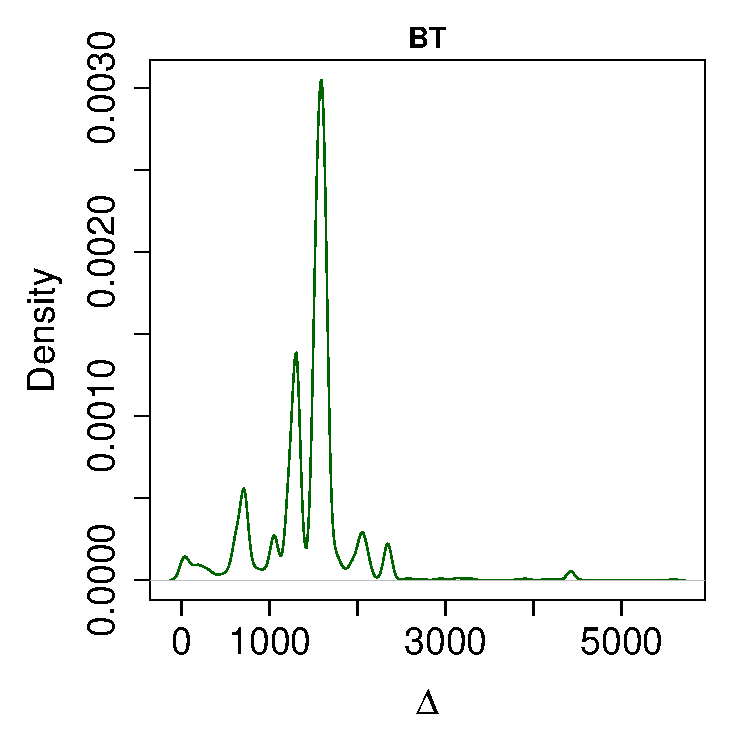
\includegraphics[width=0.2249\textwidth]{imgs/BT-unblock-dist}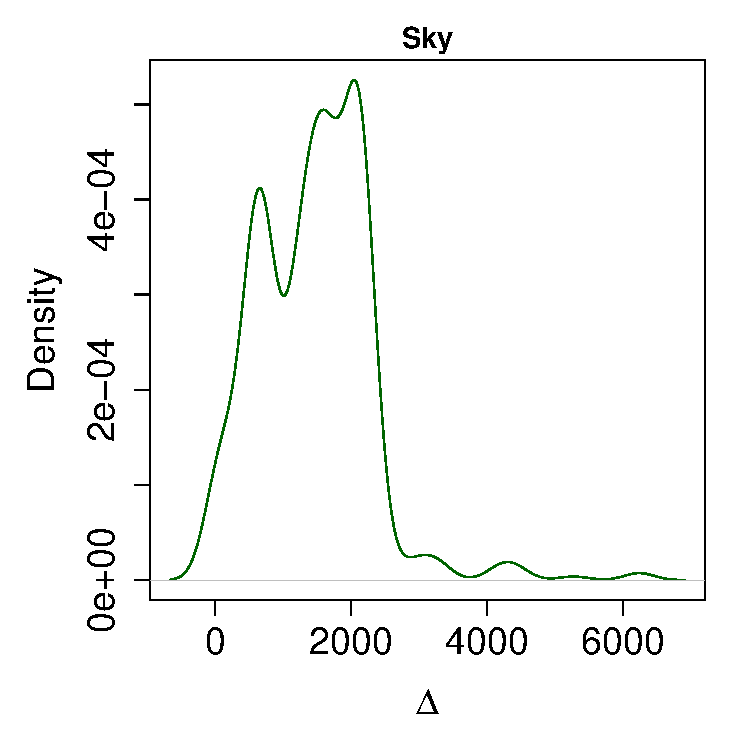
\includegraphics[width=0.2249\textwidth]{imgs/Sky-unblock-dist}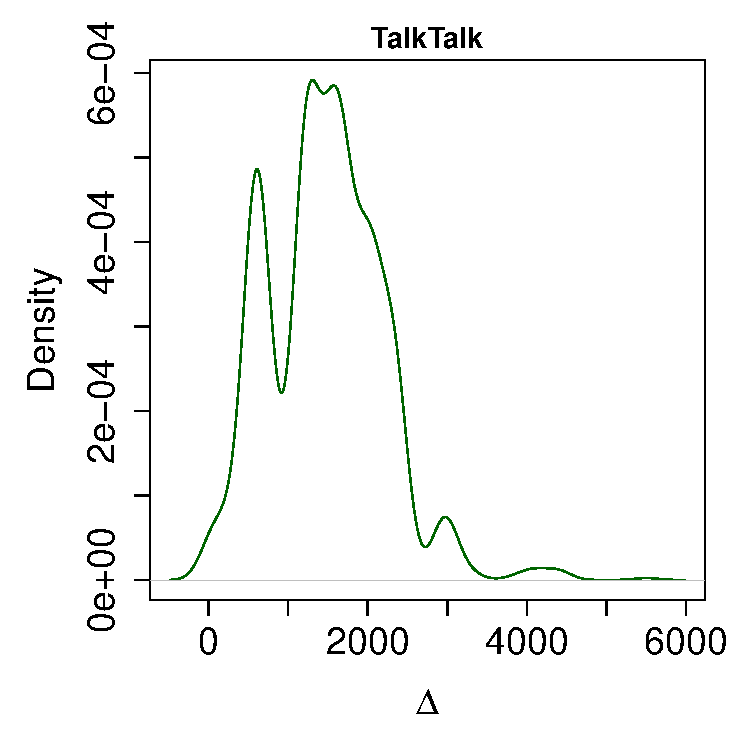
\includegraphics[width=0.2249\textwidth]{imgs/TalkTalk-unblock-dist}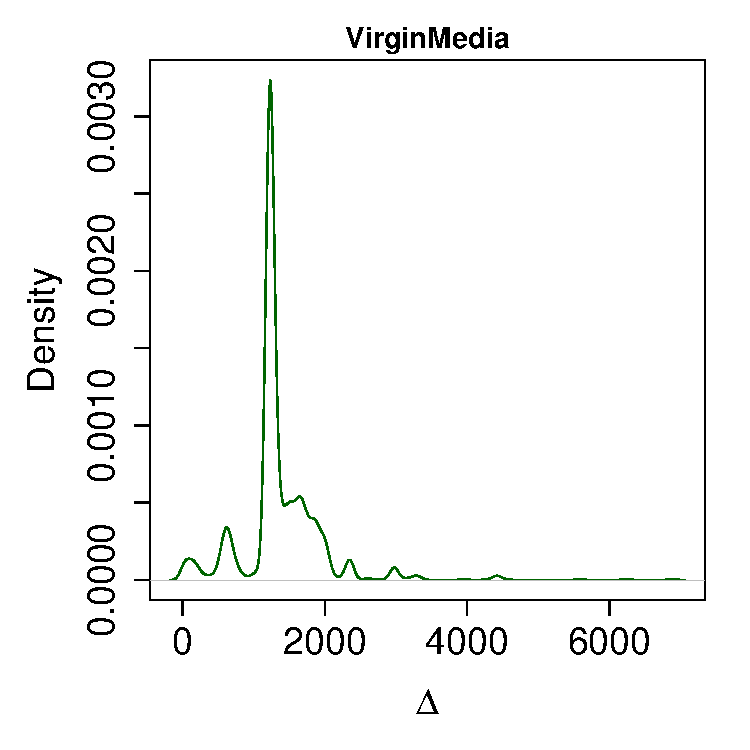
\includegraphics[width=0.2249\textwidth]{imgs/VirginMedia-unblock-dist}

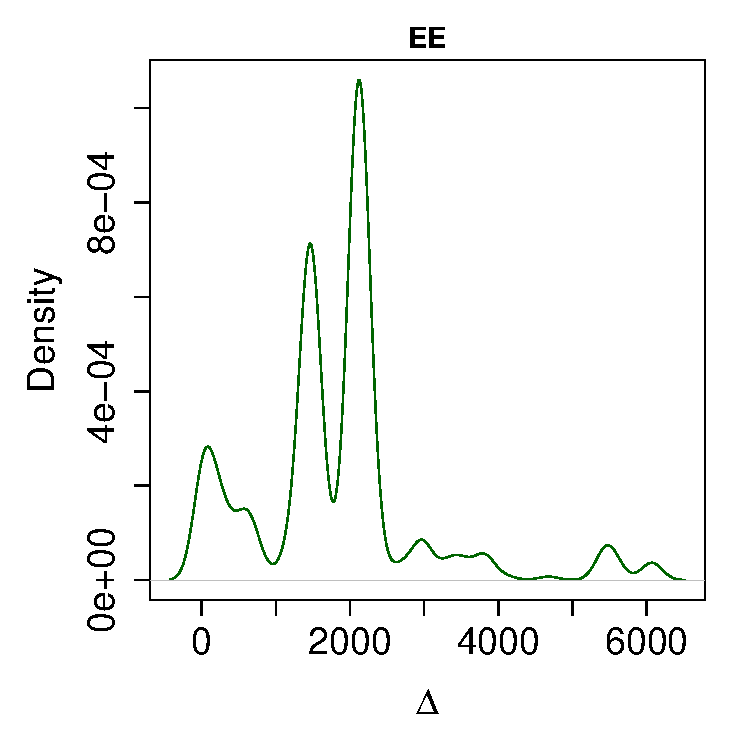
\includegraphics[width=0.2249\textwidth]{imgs/EE-unblock-dist}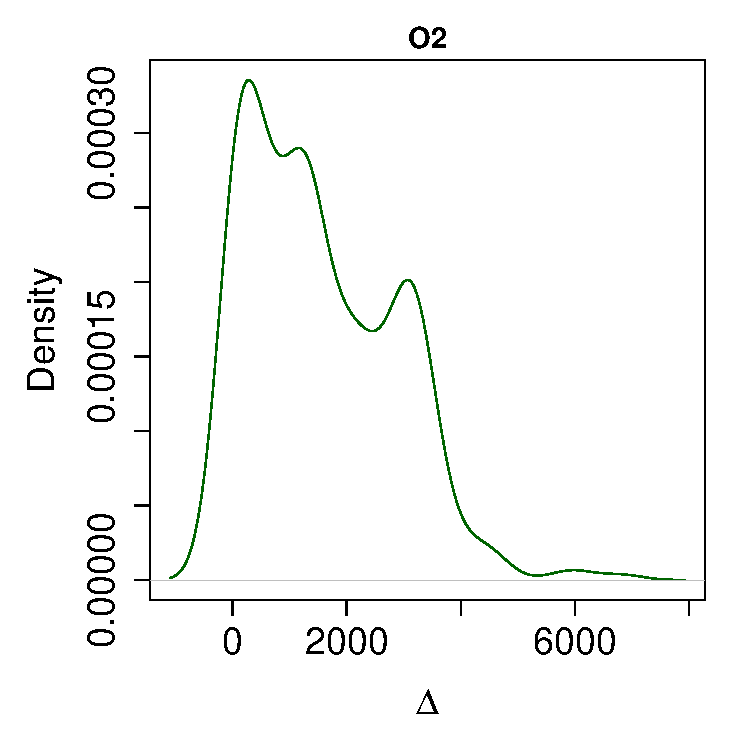
\includegraphics[width=0.2249\textwidth]{imgs/O2-unblock-dist}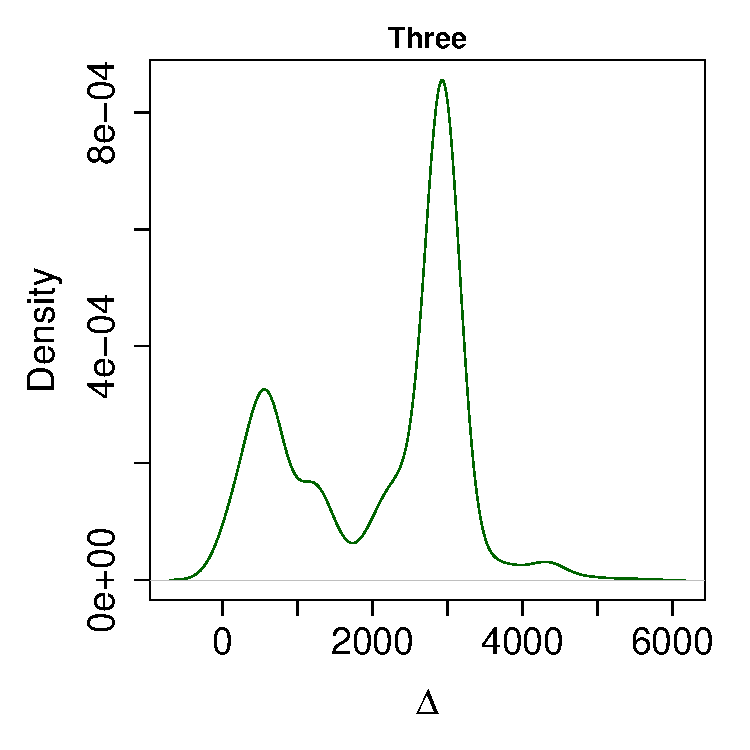
\includegraphics[width=0.2249\textwidth]{imgs/Three-unblock-dist}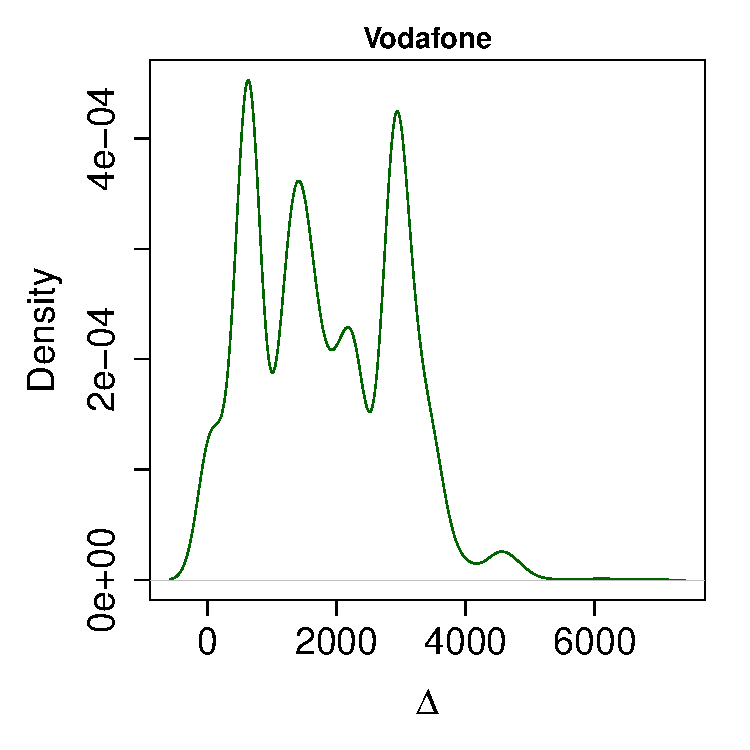
\includegraphics[width=0.2249\textwidth]{imgs/Vodafone-unblock-dist}

\label{fig:isps-unblock-dist}
\end{figure}



%%%%%% Section
\section*{Study Limitations}


\subsection*{Measurement of Blocks}
-Defend the approach of analysing which requests were fulfilled - this can contain duplicate URLs (some of which were blocked, and some of which were not)
--This can lead to repeated URLs in the lists of false/true positives and negatives
--We counteract this by using sets to restrict each URL to one occurrence per set

-Explain possible limitations with the actual probe system itself.


\subsection*{Limitations of Pseudo-Classifiers}
Limitations of this approach:
-Relies on the classification of sites within DMOZ as being correct
-Coverage of the DMOZ categories - as this is manually curated we only cover a \% of the URLs in total that have been aligned with categories

-Use of DMOZ categories is not without errors:
--E.g. the URL http://www.vin-gastronomie.com/ is not classed as should be blocked in the gold standard as its category is ''World: Francais: Regional: Europe: France: Regions: Haute-Normandie: Eure: Commerce et economie: Gastronomie et alimentation', however the page describes wine brands

-Potential improvements:
--Classifying content of the page to mine topics discussed therein - i.e. basic semantic analysis of the content
--Filtering out categories of sites which may introduce noise into the results, and not counting them at all (e.g. those related to gastronomy).


\section*{Findings and Implications}


\section*{Conclusions and Future Work}





\begin{backmatter}

\section*{Competing interests}
  The authors declare that they have no competing interests.

\section*{Acknowledgements}
Open Rights Group for providing the data and engineering the solution


% if your bibliography is in bibtex format, use those commands:
\bibliographystyle{bmc-mathphys} % Style BST file
\bibliography{bmc_article}      % Bibliography file (usually '*.bib' )



\end{backmatter}
\end{document}
